\section{Incidence across cohorts}
\label{sec:incidence}

The aggregate results hide who gains and who loses. The model has eighty annual cohorts and seven lifetime-earnings groups, so the same runs give incidence by birth cohort and by group. Representative-agent and two-group AI models cannot report this. The results below are conditional on the model's welfare measure, its transfer rule, its wealth distribution and its treatment of public debt. The section reports each of these with the size of its effect where the runs allow.

\paragraph{Measure.} Household utility in OG-Core has three parts: constant-relative-risk-aversion utility of consumption ($\sigma = \genSigma{}$), an elliptical utility of leisure, and a warm-glow utility of the assets left as a bequest (weight $\chi^b = \genChiB{}$, scaled by the probability of dying). For each birth cohort $b$ and lifetime-earnings group $j$, I compute remaining lifetime utility in the baseline and in each scenario from the household paths of the solves themselves: consumption, labour supply and assets by year, age and group. Future periods are discounted by $\beta = \genBetaAnnual{}$, the survival probabilities and the growth adjustment $e^{g_y(1-\sigma)}$ that OG-Core's detrended problem implies; the adjustment is the same in every arm. The welfare change $\lambda_{b,j}$ is the constant percentage change in the baseline's consumption and bequests, in every remaining year, that gives the household the scenario's remaining lifetime utility, with labour supply held at its baseline path. Cohorts alive in \genStartYear{} are measured over their remaining lives from \genStartYear{}, when the scenario is announced, and later cohorts over their whole lives. Each closure is measured against its own baseline. Because the change is announced in \genStartYear{} under perfect foresight, the measure includes the anticipation response of that year (Section~\ref{sec:results-anticipation}).

Three checks tie the measure to the aggregates. The household paths, weighted by the population and group shares, reproduce the results files' consumption gaps in every year from \genStartYear{} to \genEndYear{}, for both arms at both closures (to 0.001 percentage points). Comparing the baseline with itself gives zero, and the baseline with consumption and bequests 1 per cent higher gives exactly 1 per cent. The solved transition path ends in \genCevTUseLastYear{}, before the economy reaches its steady state. Later years are filled with each arm's last age profile; using each arm's steady state instead moves no cohort born by \genCevLastBirthShown{} by more than \genCevContinuationMaxDiff{} percentage points.

The groups are percentiles of lifetime earnings: 0--25, 25--50, 50--70, 70--80, 80--90, 90--99 and the top 1 per cent. They are not income deciles.

\paragraph{Results.} Figure~\ref{fig:cohorts} shows $\lambda_{b,j}$ by birth year for the bottom 25 per cent, the 50th--70th percentile group and the top 1 per cent, with the average over all groups.

\begin{figure}[htbp]
\centering
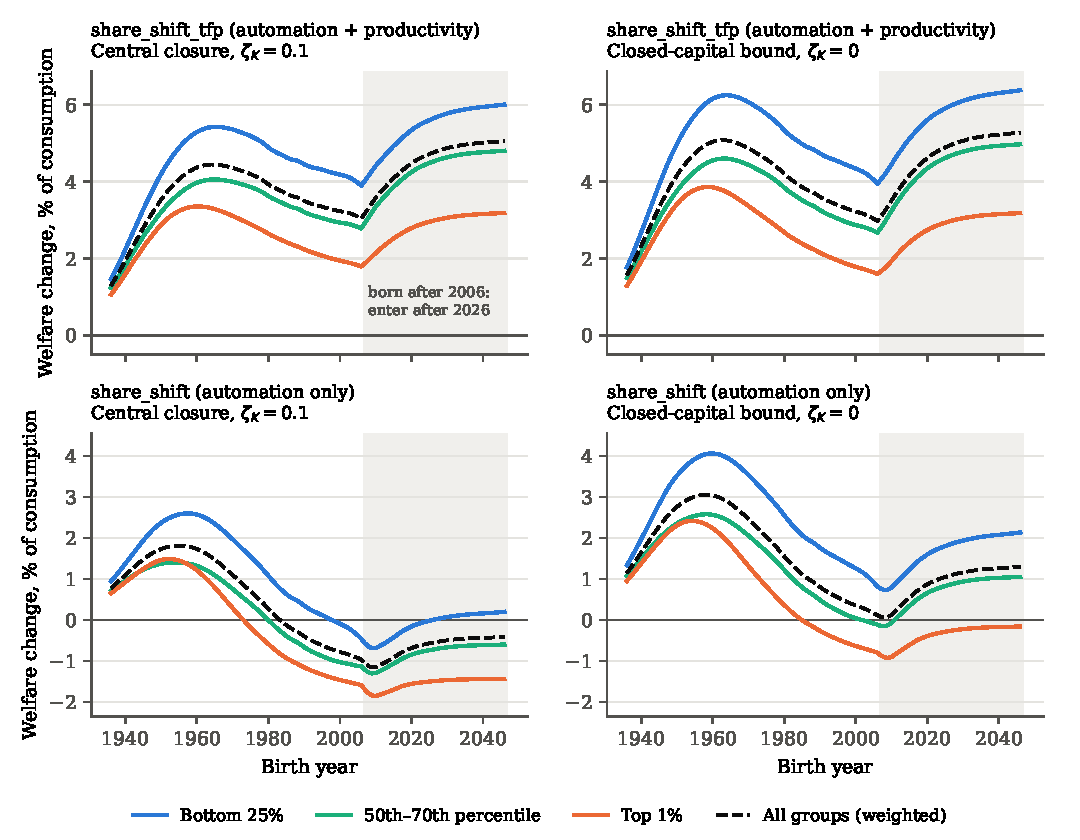
\includegraphics[width=\textwidth]{figures/cohort_cev.pdf}
\caption{Welfare change by birth cohort and lifetime-earnings group, per cent of consumption}
\label{fig:cohorts}
\par\medskip
\begin{minipage}{0.95\textwidth}
\footnotesize \emph{Notes:} consumption-and-bequest equivalent of each scenario's remaining lifetime utility, against the baseline at the same closure. Utility counts consumption, leisure and bequests (Table~\ref{tab:cevparts} separates them), and the extra public borrowing in \ShareShift{} is charged to no household. Cohorts born up to \genCevLastBirthShown{}; the shaded cohorts enter the model (at age 20) after \genStartYear{}. ``All groups'' weights the seven groups by their population shares. Source: \texttt{analysis/rerun/cohorts/}, computed by \texttt{paper/cohort\_welfare.py}.
\end{minipage}
\end{figure}

\begin{itemize}
\item \emph{\ShareShiftTfp{}.} No cohort or group loses at either closure, apart from a change of less than 0.01 per cent for the oldest cohort at the central closure. Averaged over the cohorts alive in \genStartYear{}, the welfare gain is \genShareShiftTfpCevAliveMeanCentral{} per cent at the central closure and \genShareShiftTfpCevAliveMeanBound{} per cent at the bound. Among those alive, it is largest for people aged about 60 in \genStartYear{} (\genShareShiftTfpCevAgeSixtyCentral{} per cent), who hold the most assets when the return rises and receive transfers that rise with GDP. It is smallest for those aged 20 (\genShareShiftTfpCevAgeTwentyCentral{} per cent), who hold no assets when the return rises and work through years in which the real wage is below the baseline (until the early 2030s at the central closure). Cohorts born in \genCevLastBirthShown{} gain \genShareShiftTfpCevBornFortySixCentral{} per cent.
\item \emph{\ShareShift{}.} The sign depends on age. At the central closure, cohorts aged 60 in \genStartYear{} gain \genShareShiftCevAgeSixtyCentral{} per cent, because the return on their assets rises (by \genShareShiftInterestChangeBpCentral{} basis points in \genEndYear{}) and the lower wage matters little to them. The group average turns negative for cohorts born from \genShareShiftCevFirstNegBirthCentral{}: the change is \genShareShiftCevAgeTwentyCentral{} per cent for those aged 20 in \genStartYear{} and \genShareShiftCevBornFortySixCentral{} per cent for cohorts born in \genCevLastBirthShown{}, against a real wage \genShareShiftWageGapThirtyCentralAbs{} per cent lower in \genEndYear{}. The losses are smaller than the wage fall for four reasons. Labour is only part of lifetime income. Transfers are a fixed share of an unchanged GDP, so they do not fall with wages. Households take part of the change as leisure and as higher asset holdings, both of which the measure values. And households pay less tax and receive more interest on government debt, while the extra public borrowing is charged to no one (see below).
\item \emph{Across lifetime-earnings groups.} In both scenarios the bottom 25 per cent fare better than the top 1 per cent in every cohort. For cohorts born in \genCevLastBirthShown{} at the central closure the gap is \genShareShiftTfpCevBornFortySixBottomCentral{} against \genShareShiftTfpCevBornFortySixTopOneCentral{} per cent in \ShareShiftTfp{} and \genShareShiftCevBornFortySixBottomCentral{} against \genShareShiftCevBornFortySixTopOneCentral{} per cent in \ShareShift{}. This ranking follows from how the model distributes income across groups. In the baseline in \genEndYear{}, before tax, the bottom group draws \genGrpLabourIncBottom{} per cent of its income from labour earnings against \genGrpLabourIncTopOne{} per cent for the top 1 per cent, \genGrpTransferIncBottom{} against \genGrpTransferIncTopOne{} per cent from lump-sum transfers, and \genGrpCapBeqIncBottom{} against \genGrpCapBeqIncTopOne{} per cent from capital income and bequests received. Two of these differences are modelling assumptions.
\begin{itemize}
\item \emph{Transfers.} Lump-sum transfers are the same amount per head for every household and a fixed share of GDP. They do not fall when wages fall, and in \ShareShiftTfp{} they rise with GDP. A rule that tied transfers to wages would remove part of the bottom group's advantage.
\item \emph{Wealth.} Household wealth in the model is spread more evenly across the groups than earnings are. The bottom 25 per cent hold \genGrpWealthShareBottom{} per cent of wealth and receive \genGrpEarnShareBottom{} per cent of labour earnings; the top 10 per cent hold \genGrpWealthShareTopTen{} per cent of wealth and receive \genGrpEarnShareTopTen{} per cent of earnings. Every group has the same discount factor, and bequests are shared equally within each group. So a higher return on capital reaches the bottom group at least as much as the top one. UK wealth is far more concentrated than this: the wealthiest tenth of households held 43 per cent of household wealth in 2018--20 and the bottom half 9 per cent \citep{ons2022wealth}. Those figures rank households by wealth, not lifetime earnings, so they are not like for like, but the model was not calibrated to them. In \citet{moll2022} the concentration of capital income is a main channel from automation to inequality, and that channel is weak here.
\end{itemize}
The ranking is therefore a property of the model's transfer rule and wealth distribution. It is not evidence that automation would favour lower earners in the UK.
\item \emph{Across closures.} Cohorts alive in \genStartYear{} gain more at the bound than at the central closure in both scenarios (\genShareShiftTfpCevAliveMeanBound{} against \genShareShiftTfpCevAliveMeanCentral{} per cent in \ShareShiftTfp{}, even though its GNI gain is smaller there, and \genShareShiftCevAliveMeanBound{} against \genShareShiftCevAliveMeanCentral{} per cent in \ShareShift{}). With the capital account closed to private capital, residents finance all of the extra capital, the return rises further and residents receive all of it. At the central closure foreign owners supply most of the extra capital and receive its return. In \ShareShift{} at the bound the group average is positive for every cohort born by \genCevLastBirthShown{}, and only the higher groups among the younger cohorts lose.
\end{itemize}

\paragraph{How the change is taken.} The measure counts consumption, leisure and bequests together. Table~\ref{tab:cevparts} switches one of the three at a time from the baseline's path to the scenario's.

\begin{table}[htbp]
\centering
\caption{The welfare change by the part of utility that moves, per cent of consumption}
\label{tab:cevparts}
\small
\begin{tabular}{lrrrr}
\toprule
 & \multicolumn{2}{c}{\ShareShiftTfp{}} & \multicolumn{2}{c}{\ShareShift{}} \\
\cmidrule(lr){2-3}\cmidrule(lr){4-5}
 & $\zetaK = \genZetaKCentral{}$ & $\zetaK = \genZetaKBound{}$ & $\zetaK = \genZetaKCentral{}$ & $\zetaK = \genZetaKBound{}$ \\
\midrule
\emph{Alive in \genStartYear{}, average} \\
Consumption only & \genShareShiftTfpCevPartConsAliveMeanCentral{} & \genShareShiftTfpCevPartConsAliveMeanBound{} & \genShareShiftCevPartConsAliveMeanCentral{} & \genShareShiftCevPartConsAliveMeanBound{} \\
Leisure only & \genShareShiftTfpCevPartLeisureAliveMeanCentral{} & \genShareShiftTfpCevPartLeisureAliveMeanBound{} & \genShareShiftCevPartLeisureAliveMeanCentral{} & \genShareShiftCevPartLeisureAliveMeanBound{} \\
Bequests only & \genShareShiftTfpCevPartBeqAliveMeanCentral{} & \genShareShiftTfpCevPartBeqAliveMeanBound{} & \genShareShiftCevPartBeqAliveMeanCentral{} & \genShareShiftCevPartBeqAliveMeanBound{} \\
All three (the measure) & \genShareShiftTfpCevAliveMeanCentral{} & \genShareShiftTfpCevAliveMeanBound{} & \genShareShiftCevAliveMeanCentral{} & \genShareShiftCevAliveMeanBound{} \\[0.15cm]
\emph{Aged 60 in \genStartYear{}} \\
Consumption only & \genShareShiftTfpCevPartConsAgeSixtyCentral{} & \genShareShiftTfpCevPartConsAgeSixtyBound{} & \genShareShiftCevPartConsAgeSixtyCentral{} & \genShareShiftCevPartConsAgeSixtyBound{} \\
Leisure only & \genShareShiftTfpCevPartLeisureAgeSixtyCentral{} & \genShareShiftTfpCevPartLeisureAgeSixtyBound{} & \genShareShiftCevPartLeisureAgeSixtyCentral{} & \genShareShiftCevPartLeisureAgeSixtyBound{} \\
Bequests only & \genShareShiftTfpCevPartBeqAgeSixtyCentral{} & \genShareShiftTfpCevPartBeqAgeSixtyBound{} & \genShareShiftCevPartBeqAgeSixtyCentral{} & \genShareShiftCevPartBeqAgeSixtyBound{} \\
All three (the measure) & \genShareShiftTfpCevAgeSixtyCentral{} & \genShareShiftTfpCevAgeSixtyBound{} & \genShareShiftCevAgeSixtyCentral{} & \genShareShiftCevAgeSixtyBound{} \\[0.15cm]
\emph{Aged 20 in \genStartYear{}} \\
Consumption only & \genShareShiftTfpCevPartConsAgeTwentyCentral{} & \genShareShiftTfpCevPartConsAgeTwentyBound{} & \genShareShiftCevPartConsAgeTwentyCentral{} & \genShareShiftCevPartConsAgeTwentyBound{} \\
Leisure only & \genShareShiftTfpCevPartLeisureAgeTwentyCentral{} & \genShareShiftTfpCevPartLeisureAgeTwentyBound{} & \genShareShiftCevPartLeisureAgeTwentyCentral{} & \genShareShiftCevPartLeisureAgeTwentyBound{} \\
Bequests only & \genShareShiftTfpCevPartBeqAgeTwentyCentral{} & \genShareShiftTfpCevPartBeqAgeTwentyBound{} & \genShareShiftCevPartBeqAgeTwentyCentral{} & \genShareShiftCevPartBeqAgeTwentyBound{} \\
All three (the measure) & \genShareShiftTfpCevAgeTwentyCentral{} & \genShareShiftTfpCevAgeTwentyBound{} & \genShareShiftCevAgeTwentyCentral{} & \genShareShiftCevAgeTwentyBound{} \\
\bottomrule
\end{tabular}
\par\medskip
\begin{minipage}{0.95\textwidth}
\footnotesize \emph{Notes:} each ``only'' row is the consumption-and-bequest equivalent when that part of utility alone (consumption, labour supply, or assets carried forward) follows the scenario's path and the other two follow the baseline's. The parts do not sum exactly to the measure, which is not linear. Averages over the seven groups; ``alive in \genStartYear{}'' also averages over cohorts by population. Source: \texttt{analysis/rerun/cohorts/}, computed by \texttt{paper/cohort\_welfare.py}.
\end{minipage}
\end{table}

In \ShareShift{} the consumption row is negative at the central closure (\genShareShiftCevPartConsAliveMeanCentral{} per cent) and about zero at the bound (\genShareShiftCevPartConsAliveMeanBound{} per cent). Counting consumption alone, those alive in \genStartYear{} lose on average at the central closure and are about unchanged at the bound. The positive averages on the full measure (\genShareShiftCevAliveMeanCentral{} and \genShareShiftCevAliveMeanBound{} per cent) come from leisure and, more, from bequests. For those aged 20 in \genStartYear{} the consumption row is \genShareShiftCevPartConsAgeTwentyCentral{} per cent at the central closure and \genShareShiftCevPartConsAgeTwentyBound{} per cent at the bound. In \ShareShiftTfp{} all three rows are positive, and consumption accounts for less than half of the total.

The bequest term is OG-Core's warm glow. At every age a household values the assets it carries into the next year, weighted by its probability of dying, with weight $\chi^b = \genChiB{}$. When the return on capital rises households hold more assets, and the measure counts that as a gain to the holder; the same assets are later income to those who inherit them. The split describes the form in which households take the change. It is not a split by cause, because labour supply and saving are chosen. A reader who values consumption alone should use the consumption rows.

\paragraph{What the measure leaves out.} Five features of the model shape these numbers.
\begin{itemize}
\item In \ShareShift{} the extra public borrowing is charged to no household. Public borrowing is \genShareShiftBorrowGapGdpThirtyCentral{} per cent of baseline GDP higher than in the baseline in \genEndYear{} at the central closure and \genShareShiftBorrowGapGdpThirtyBound{} per cent higher at the bound, which is \genShareShiftBorrowGapConsThirtyCentral{} and \genShareShiftBorrowGapConsThirtyBound{} per cent of baseline consumption. Revenue falls as income moves from labour to capital, and the interest rate on the whole stock of debt rises with the return on capital, while spending is unchanged because GDP is. More than four-fifths of the extra borrowing reaches households, as a lower tax bill and higher interest on the gilts they hold. No tax or transfer adjusts in any run, and from \genTGoneYear{} the debt rule adjusts government consumption, which does not enter utility. Within the measure the extra borrowing is therefore a transfer to households that no cohort repays. By \genEndYear{} it is larger than the average welfare change of those alive in \genStartYear{} at either closure (\genShareShiftCevAliveMeanCentral{} and \genShareShiftCevAliveMeanBound{} per cent). The positive averages for that scenario are therefore not robust to how the budget is closed. If taxes or transfers adjusted, the figures would be lower for every cohort alive during the adjustment; by how much, and for which groups, depends on the instrument, and no run here closes the budget on households.
\item Government consumption does not enter utility. In \ShareShiftTfp{} government consumption rises with GDP, by more than the extra public borrowing in that scenario (\genShareShiftTfpBorrowGapConsThirtyCentral{} and \genShareShiftTfpBorrowGapConsThirtyBound{} per cent of consumption in \genEndYear{}), and households pay more tax than in the baseline. The measure counts the extra public consumption as no gain, and a cut under the debt rule from \genTGoneYear{} as no loss.
\item Perfect foresight. Households know the whole path from \genStartYear{} and re-plan at once. A model in which the change is learned gradually would leave the cohorts alive in \genStartYear{} less time to adjust. No run tests this.
\item Leisure is valued. Labour supply falls in both scenarios, including among older households, who keep working in OG-Core at every age, and the extra leisure counts as a gain.
\item Bequests are valued by the giver. Scaling consumption alone instead of consumption and bequests together gives much larger figures for older cohorts, because their remaining bequest utility exceeds their remaining consumption utility: for cohorts aged 80 in \genStartYear{} at the central closure, \genShareShiftTfpCevConsOnlyAgeEightyCentral{} against \genShareShiftTfpCevAgeEightyCentral{} per cent in \ShareShiftTfp{}, and \genShareShiftCevConsOnlyAgeEightyCentral{} against \genShareShiftCevAgeEightyCentral{} per cent in \ShareShift{}. For the youngest and future cohorts the two measures differ little.
\end{itemize}
The aggregate consumption gap in \genEndYear{} is small (\genShareShiftTfpConsumptionGapThirty{} per cent in \ShareShiftTfp{} at the central closure) while most welfare gains are several per cent. Both are correct. Consumption is below the baseline in \genStartYear--2029 and above it afterwards, rising further as capital accumulates, and the welfare measure also counts leisure and bequests.
